\chapter{Experimental Facilities}

\section{The Relativistic Heavy Ion Collider (RHIC)}

\begin{figure}
  \begin{center}
    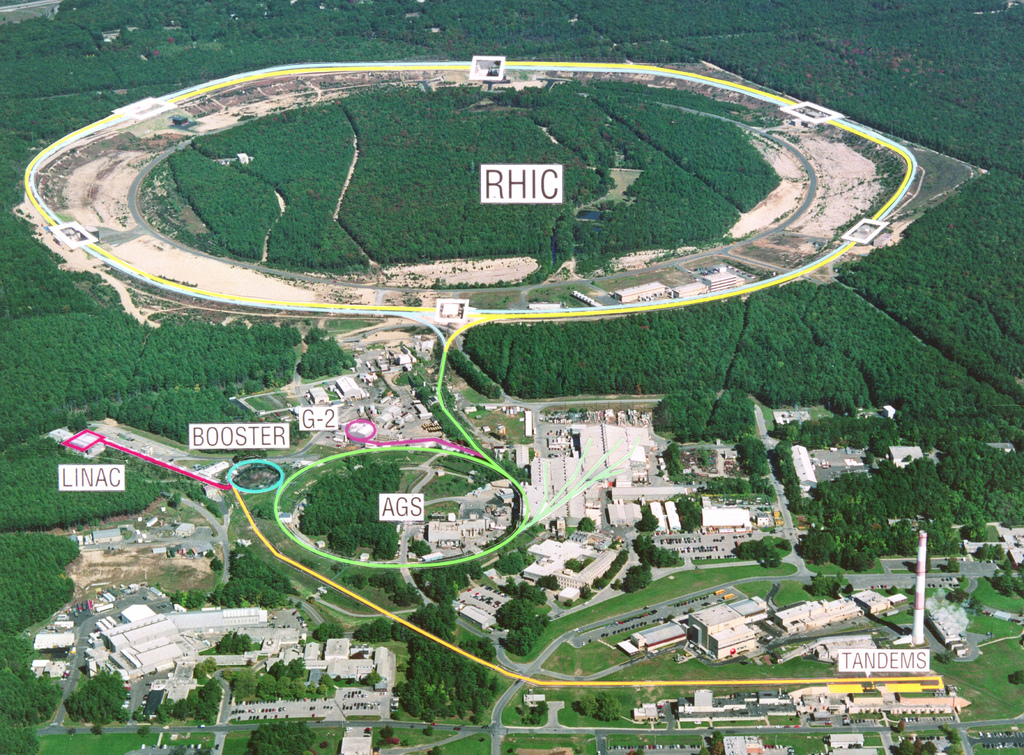
\includegraphics[width=0.8\textwidth]{figures/rhic-from-above}
  \end{center}
  \caption{}
  \label{fig:rhic}
\end{figure}

The Relativistic Heavy Ion Collider (RHIC) is an intersecting storage ring located at Brookhaven National Laboratory in Upton, New York.  Unusually versatile for a collider, RHIC uses two independent superconducting rings to collide beams of ions with mass numbers separately ranging from one to 197.  Recent beam configurations have included protons on protons, deuterons on gold, copper on copper, and gold on gold.  Figure \ref{fig:rhic} shows a schematic view of the RHIC accelerator complex.  The main RHIC ring has a 3.8 kilometer circumference and is comprised of six straight sections and six curved sections.  Collisions between the beams occur in the middle of each straight section, and four experimental halls are situated at the two (BRAHMS), six (STAR), eight (PHENIX), and ten o'clock (PHOBOS) positions.

RHIC relies on a complex of smaller accelerators to prepare ion beams for injection into the main ring.  This work focuses on the systems used to polarize and accelerate beams of protons, thus avoiding further discussion of the Tandem Van de Graff generator used exclusively in heavy ion operations.  Polarized protons are produced using OPPIS \cite{Zelenski:2002gb, Zelenski:2008zza}, an optically-pumped polarized ion source which typically generates 0.5mA, 400 $\mu$s pulses of ions, corresponding to $\mathrm{9x10^{11}}$ ions per pulse.  The pulsed nature of the beam is crucial to delivering the RHIC design luminosity of $\mathrm{2x10^{32}~cm^{-2}~s^{-1}}$. OPPIS polarizes protons by passing them through a rubidium vapor pumped with circularly polarized laser light in a strong magnetic field.  The $\mathrm{H^+}$ ions pick up a polarized rubidium electron through collisions in the vapor, and magnetic fields cause the electron polarization to be transferred to the nucleus.  Finally, the hydrogen atoms are ionized to $\mathrm{H^-}$ when they pass through a sodium vapor.

The pulses of 35 keV $\mathrm{H^-}$ ions produced by OPPIS are accelerated by the LINAC, Booster, and AGS on their way to RHIC.  The LINAC strips off the electrons and accelerates the protons to a kinetic energy of 200 MeV with an efficiency of approximately 50\%.  It injects the remaining $\sim \mathrm{4x10^{11}}$ ions into the Booster ring in a single bunch.  The Booster
accelerates the protons to 1.5 GeV and passes them on to the Alternating Gradient Synchrotron (AGS), which accelerates them to the RHIC injection energy of 25 GeV.  RHIC accelerates the $\sim \mathrm{4x10^{11}}$ to the desired collision energy, which can range from 30 GeV to 250 GeV.  This work analyzes data collected with a beam energy of 100 GeV.  More details of the RHIC accelerator complex are available in references \cite{Harrison:2003sb, Hahn:2003sc, Alekseev:2003sk}.

\subsection{Spin Dynamics and Siberian Snakes}

The evolution of the spin direction of a beam of polarized protons in external magnetic fields is governed by the Thomas-BMT equation \cite{Thomas:1927yu, Bargmann:1959gz},
%
\begin{equation}
  \frac{d\vec{P}}{dt} = -\left(\frac{e}{\gamma m}\right)[(G\gamma + 1) \vec{B}_{\perp} + (G + 1) \vec{B}_{\parallel}] \times \vec{P}.
\end{equation}
%
Comparing this equation with the Lorentz force equation governing the orbital motion,
%
\begin{equation}
  \frac{d\vec{v}}{dt} = -\left(\frac{e}{\gamma m}\right)[\vec{B}_{\perp}] \times \vec{v},
\end{equation}
%
one realizes that, in a pure vertical magnetic field, the spin rotates G$\gamma$ + 1 times faster than the orbital motion. This factor, referred to as the spin tune $\nu_{sp}$, gives the number of full spin precessions for every orbit.

An accelerating beam in a storage ring encounters depolarizing resonances whenever the spin tune is equal to an integer multiple of the frequency with which a spin-depolarizing magnetic field is encountered.  In the simplest case, a depolarizing field can be introduced by a magnet error or misalignment.  For these \textit{imperfection resonances}, the resonance condition is just $G\gamma = n$.  If $G\gamma$ is non-integral, the beam sees the depolarizing field at a different point in its precession on each revolution, and the effects tend to cancel out.  The focusing fields themselves can also be a source of depolarization; for these \textit{intrinsic resonances} the resonance condition is $G\gamma = kP \pm \nu_y$, where $k$ is an integer, $\nu_y$ is the vertical betatron tune, and $P$ is the superperiodicity.

The stable spin direction in an accelerating beam normally coincides with the vertical magnetic field, but near a resonance, it gets perturbed away from the vertical by the resonance driving fields.  The polarization loss when a beam is accelerated through one of these resonances can be calculated analytically \cite{}:
%
\begin{equation}
  \frac{P_f}{P_i} = 2 e^{-\pi |\epsilon|^2 / 2\alpha} -1.
\end{equation}
%
Here $\epsilon$ is the resonance strength and $\alpha$ is the change of the spin tune per radian of the orbit angle.  When the beam is slowly accelerated ($\alpha << |\epsilon|^2$) the stable spin direction changes adiabatically and the result is a spin flip.  In contrast, techniques such as betatron tune jump serve to make $|\epsilon|^2 << \alpha$ and thus preserve the polarization through the resonance.  At high energies, the number and strength of the resonances encountered make these traditional techniques impractical.


% spin rotators

% dumping the beam

% cogging / bunch patterns

\subsection{Polarimetry Systems}

\cite{Jinnouchi:2004up} % CNI
\cite{Okada:2006dd} % H-jet

% 2 paragraphs on CNI, barely anything on H-jet

\section{The Solenoidal Tracker at RHIC (STAR)}

\cite{Ackermann:2002ad} % STAR detector overview

\begin{figure}
  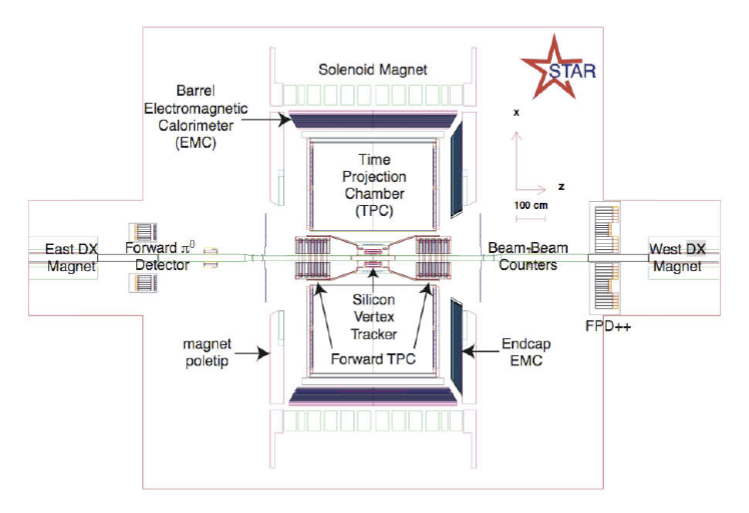
\includegraphics[width=1.0\textwidth]{figures/star-schematic}
  \caption{}
  \label{fig:star-schematic}
\end{figure}

\subsection{Trigger Detectors}

\subsection{The Barrel Electromagnetic Calorimeter}

\cite{Beddo:2002zx} % BEMC overview

\subsection{The Time Projection Chamber}

\cite{Anderson:2003ur} % TPC overview

\begin{figure}
  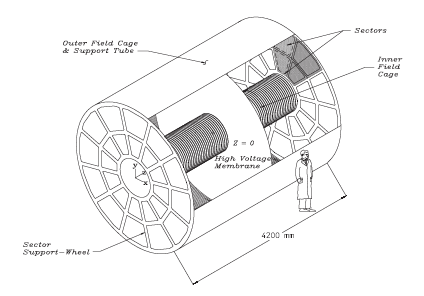
\includegraphics[width=1.0\textwidth]{figures/tpc}
  \caption{}
  \label{fig:tpc}
\end{figure}

\subsection{Computing Facilities}
